\documentclass[11pt,a4paper]{article}
\usepackage[utf8]{inputenc}
\usepackage[T1]{fontenc}
\usepackage[spanish]{babel}
\usepackage[margin=2.3cm]{geometry}
\usepackage{graphicx}
\usepackage{booktabs}
\usepackage{amsmath}
\usepackage{float}
\usepackage{hyperref}

\title{Laboratorio 5: DBSCAN + KDTree}
\author{Gonzalo Sumina Quispe\\Estructuras de Datos Avanzadas -- UCSP}
\date{25 de noviembre de 2026}

\begin{document}
	\maketitle
	
	\section{Implementación y datasets}
	Se implementó en C++ el algoritmo DBSCAN siguiendo el pseudocódigo del enunciado (etiqueta $0$ = sin procesar, $-1$ = ruido, $1..K$ = cluster). Ambas versiones comparten exactamente el mismo código del algoritmo; solo cambia la función de consulta por rango:
	\begin{itemize}
		\item \textbf{Clásica:} recorre los $n$ puntos para cada consulta.
		\item \textbf{KDTree:} usa un árbol k-d construido con la mediana en cada nivel.
	\end{itemize}
	En todos los experimentos ambas versiones produjeron etiquetas idénticas.
	
	\paragraph{Datasets.} Se generaron con scikit-learn y se estandarizaron: (a) \texttt{moons\_2d}, 10\,000 puntos en 2D con forma de dos lunas y ruido 0.07; (b) \texttt{blobs\_6d}, 5\,000 puntos en 6D con 4 grupos. El de 6D se visualiza reduciéndolo a 2D con PCA. El Silhouette Score se calculó en Python con \texttt{sklearn.metrics.silhouette\_score}, excluyendo los outliers (etiqueta $-1$).
	
	\section{Resultados con distintos hiperparámetros}
	\begin{table}[H]
		\centering
		\small
		\begin{tabular}{lrrrrrrrr}
			\toprule
			Dataset & $\varepsilon$ & minPts & Clusters & Outliers & Silhouette & $t_{cl}$ (s) & $t_{kd}$ (s) & Aceleración \\
			\midrule
			moons\_2d & 0.05 & 5  & 3 & 275  & 0.262 & 0.281 & 0.017 & 16.4$\times$ \\
			moons\_2d & 0.10 & 5  & 2 & 14   & 0.390 & 0.288 & 0.029 & 10.0$\times$ \\
			moons\_2d & 0.20 & 5  & 2 & 0    & 0.389 & 0.276 & 0.059 & 4.7$\times$ \\
			moons\_2d & 0.10 & 30 & 2 & 124  & 0.390 & 0.297 & 0.033 & 8.9$\times$ \\
			\midrule
			blobs\_6d & 0.3 & 10 & 6 & 2515 & 0.446 & 0.186 & 0.026 & 7.3$\times$ \\
			blobs\_6d & 0.6 & 10 & 4 & 20   & 0.665 & 0.146 & 0.063 & 2.3$\times$ \\
			blobs\_6d & 1.0 & 10 & 4 & 0    & 0.663 & 0.191 & 0.097 & 2.0$\times$ \\
			blobs\_6d & 0.6 & 40 & 4 & 66   & 0.668 & 0.150 & 0.080 & 1.9$\times$ \\
			\bottomrule
		\end{tabular}
		\caption{Resultados por combinación de hiperparámetros. $t_{cl}$: DBSCAN clásico, $t_{kd}$: DBSCAN con KDTree (incluye la construcción del árbol).}
	\end{table}
	
	\begin{figure}[H]
		\centering
		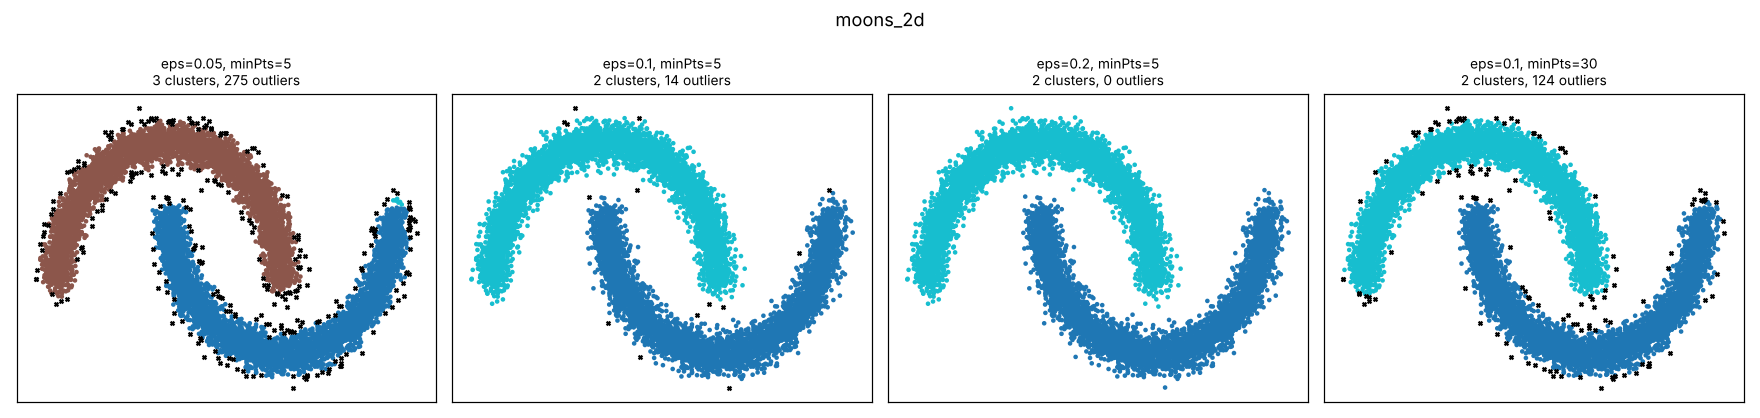
\includegraphics[width=\textwidth]{resultados/clusters_moons_2d.png}
		\caption{Clusterización de \texttt{moons\_2d} (los outliers se marcan con una cruz negra).}
	\end{figure}
	
	\begin{figure}[H]
		\centering
		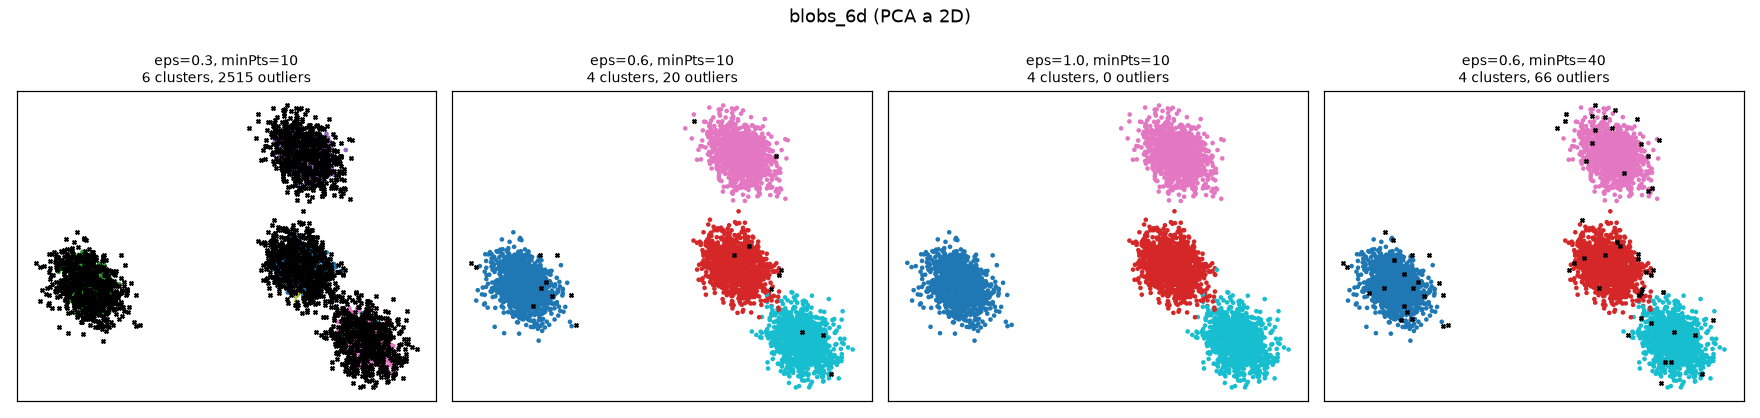
\includegraphics[width=\textwidth]{resultados/clusters_blobs_6d.png}
		\caption{Clusterización de \texttt{blobs\_6d}, proyectada a 2D con PCA.}
	\end{figure}
	
	\paragraph{Análisis.} En \texttt{moons\_2d}, $\varepsilon=0.05$ es demasiado pequeño: fragmenta las lunas en 3 clusters y marca 275 outliers. Con $\varepsilon=0.1$ se recuperan las 2 lunas con solo 14 outliers. Con $\varepsilon=0.2$ ya no hay outliers, pero el valor es lo bastante grande como para arriesgarse a unir lunas distintas. Subir minPts a 30 con $\varepsilon=0.1$ mantiene los 2 clusters, pero convierte más puntos en ruido (124).
	
	En \texttt{blobs\_6d}, $\varepsilon=0.3$ es demasiado pequeño (6 clusters, 2515 outliers). Con $\varepsilon=0.6$ se recuperan los 4 grupos reales, con silueta 0.665 (0.668 con minPts $=40$, a costa de más outliers). Con $\varepsilon=1.0$ no queda ruido y la silueta casi no cambia.
	
	La silueta favorece clusters convexos, por eso en las lunas (no convexas) sus valores ($\approx 0.39$) son bajos aunque la clusterización sea correcta.
	
	\section{Comparación de tiempos}
	El KDTree fue más rápido en todos los casos de la tabla anterior (entre $1.9\times$ y $16.4\times$). Para ver cómo escala con $n$ se usó \texttt{moons} en 2D con $\varepsilon=0.1$ y minPts $=5$:
	
	\begin{table}[H]
		\centering
		\begin{tabular}{rrr}
			\toprule
			$n$ & Clásico (s) & KDTree (s) \\
			\midrule
			2\,000  & 0.009 & 0.002 \\
			5\,000  & 0.054 & 0.008 \\
			10\,000 & 0.293 & 0.032 \\
			20\,000 & 1.149 & 0.088 \\
			40\,000 & 4.571 & 0.344 \\
			\bottomrule
		\end{tabular}
		\caption{Tiempo de ejecución según el número de puntos (2D).}
	\end{table}
	
	\begin{figure}[H]
		\centering
		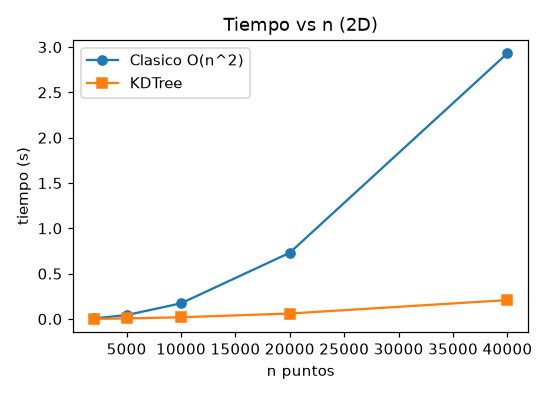
\includegraphics[width=0.6\textwidth]{resultados/tiempo_vs_n.png}
		\caption{Tiempo vs $n$ en 2D.}
	\end{figure}
	
	Al duplicar $n$, el tiempo del clásico se multiplica por aproximadamente 4 (comportamiento cuadrático), mientras que el del KDTree crece de forma cercana a $n\log n$. La construcción del árbol es una parte pequeña del tiempo total.
	
	\section{Preguntas del laboratorio}
	
	\subsection*{Complejidad computacional}
	\textbf{Clásico:} cada consulta de vecinos cuesta $O(n\cdot d)$ y se hace una por punto, luego el tiempo total es $O(n^2 d)$ y la memoria $O(n)$.
	
	\textbf{KDTree:} construir el árbol cuesta $O(n\log n)$; cada consulta por rango cuesta en promedio $O(\log n + m)$ en baja dimensión ($m$ = número de vecinos), así que el total es aproximadamente $O(n\log n)$. En el peor caso (alta dimensión o $\varepsilon$ grande) la consulta degenera a $O(n)$ y se vuelve a $O(n^2)$.
	
	\subsection*{Silhouette Score}
	Se midió y está en la columna \emph{Silhouette} de la Tabla~1: 0.390 para \texttt{moons\_2d} ($\varepsilon=0.1$, minPts $=5$) y 0.665 para \texttt{blobs\_6d} ($\varepsilon=0.6$, minPts $=10$). Va de $-1$ a $1$; valores cercanos a $1$ indican clusters compactos y bien separados.
	
	\subsection*{¿Cómo estimar un valor inicial de min\_samples?}
	Una regla práctica es $\text{minPts}\ge d+1$, y comúnmente $\text{minPts}=2d$. Para datos con ruido o muy grandes conviene subirlo (por ejemplo, entre 10 y 50). Aquí se usó 5 para 2D y 10 para 6D.
	
	\subsection*{Estrategias para optimizar $\varepsilon$ y min\_samples}
	\begin{enumerate}
		\item \textbf{Gráfico k-distance:} se ordenan las distancias de cada punto a su $k$-ésimo vecino ($k=$ minPts) y se elige $\varepsilon$ en el ``codo'' de la curva (Figura~\ref{fig:kdist}).
		\item \textbf{Búsqueda en rejilla} sobre $\varepsilon$ y minPts maximizando el Silhouette Score (o DBCV para clusters no convexos), vigilando que no quede casi todo como ruido.
		\item Revisar el número de clusters y de outliers de cada combinación.
		\item Conocimiento del dominio.
		\item Alternativas como HDBSCAN u OPTICS, que no requieren fijar $\varepsilon$.
	\end{enumerate}
	
	\begin{figure}[H]
		\centering
		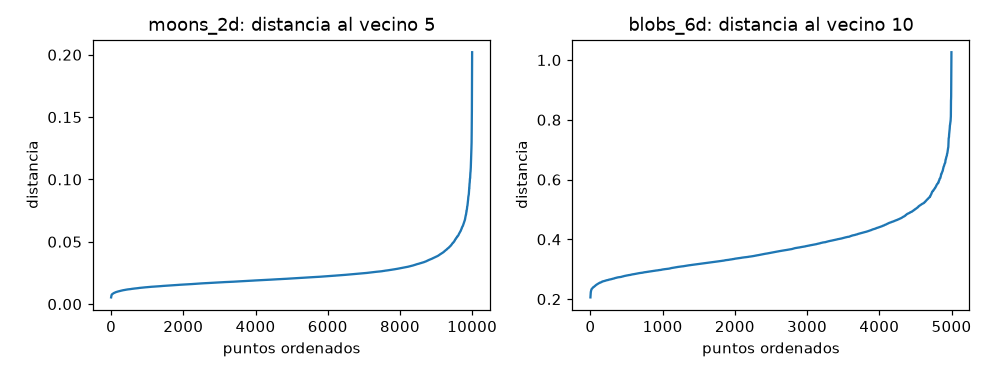
\includegraphics[width=0.9\textwidth]{resultados/kdistance.png}
		\caption{Gráfico k-distance de ambos datasets.}
		\label{fig:kdist}
	\end{figure}
	
	\subsection*{Maldición de la dimensionalidad}
	En alta dimensión las distancias entre puntos tienden a parecerse (el vecino más cercano y el más lejano quedan casi a la misma distancia), por lo que $\varepsilon$ pierde poder discriminativo: o todo queda como ruido o todo se une en un solo cluster, y la elección de $\varepsilon$ se vuelve muy sensible. Estrategias: estandarizar los datos, reducir la dimensión (PCA, t-SNE, UMAP) antes de agrupar, seleccionar características, usar distancias alternativas (coseno, Manhattan) y elegir $\varepsilon$ con el k-distance en el espacio reducido.
	
	\subsection*{Limitaciones del KDTree y alternativas}
	El KDTree pierde su ventaja cuando la dimensión es alta (como regla general, $d$ mayor que 10--20), porque la poda por hiperplanos casi no descarta ramas y se visitan casi todos los nodos; también cuando $\varepsilon$ es grande (muchos vecinos por consulta). En el experimento de dimensión (blobs de 4 grupos, $n=4000$) la ventaja bajó de $\approx 3.0\times$ en 2D a $\approx 2.2\times$ en 32D:
	
	\begin{table}[H]
		\centering
		\begin{tabular}{rrr}
			\toprule
			$d$ & Clásico (s) & KDTree (s) \\
			\midrule
			2  & 0.058 & 0.019 \\
			4  & 0.106 & 0.057 \\
			8  & 0.142 & 0.086 \\
			16 & 0.239 & 0.129 \\
			32 & 0.418 & 0.188 \\
			\bottomrule
		\end{tabular}
		\caption{Tiempo según la dimensión ($n=4000$, $\varepsilon=0.3\sqrt{d}$, minPts $=10$).}
	\end{table}
	
	\begin{figure}[H]
		\centering
		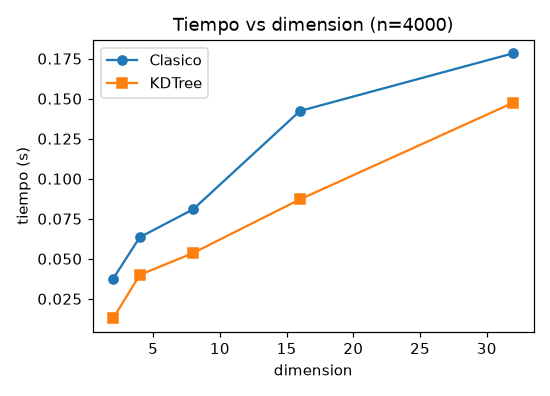
\includegraphics[width=0.6\textwidth]{resultados/tiempo_vs_dim.png}
		\caption{Tiempo vs dimensión.}
	\end{figure}
	
	Esta caída es moderada porque los datos sintéticos están muy agrupados (baja dimensión intrínseca); con datos realmente dispersos en 32D la ventaja sería menor. Alternativas: Ball Tree (mejor en dimensiones moderadas), búsqueda aproximada de vecinos (LSH, HNSW, Annoy, FAISS), reducción de dimensión previa o índices por rejilla.
	
\end{document}